\documentclass[12pt]{article}
\usepackage{times}
\usepackage{latexsym}
\usepackage{graphicx}
\usepackage{url}
\usepackage{float}
\usepackage[table,xcdraw]{xcolor}

\linespread{1}
\title{Anthropocentric Bias in Viral Genome Sequencing: Which Viruses Get Sequenced?}
\date{\today}
\author{Jacob Osborne}


\begin{document}

    \begin{titlepage}
        \begin{center}
            \vspace*{1in}
            \LARGE
            Anthropocentric Bias in Viral Genome Sequencing: Which Viruses Get Sequenced?

            \vspace*{1in}
            \large
            Jacob Osborne

            \vfill
            [DEGREE PROGRAM] \\
            Dr. Claus Wilke, Integrative Biology \\
            \today
        \end{center}
    \end{titlepage}
    
    \begin{abstract}
        The NCBI viral genomes database provides an extensive catalogue of genetic
        information from a variety of virus species. Yet, not all viruses are equal
        in their relevance to human life; there is some suspicion that those more
        directly important to our lives are significantly more likely to be
        sequenced than those that are not. To ascertain the existence and extent
        of this anthropocentric bias, a large-scale statistical analysis of the
        database was performed, and showed this was indeed the case.
        Specific patterns as to which viruses are more likely  to be sequenced
        are also documented and discussed.
    \end{abstract}

    \section{Introduction}

    The NCBI Viral Genomes database provides a large catalogue of viral genomes 
    sequenced by scientists around the world. It is the preeminent resource for
    obtaining records of viral genomes for scientific analysis.

    Yet, there is some doubt as to the extent to which the genomes catalogued
    therein can be taken as representative of viral genomes present in the
    natural world as a whole. We suspect the genomes of viruses that infect
    humans, domestic animals, and domestic plants - living things that are
    directly relevant to human life - are far more likely to be sequenced than
    the genomes of those which do not.

    The aim of this project, therefore, is to ascertain the extent of this
    anthropocentric bias in the NCBI database.

    \section{Data \& Methodology}
    
    \subsection{Overview}

    The NCBI viral genomes database does not provide information on the hosts
    of the viruses it contains records on. Thankfully, the Virus-Host Database provides
    linkages between the various NCBI databases' (including the Viral Genomes
    database) records for viruses and the records for their hosts. Therefore,
    this project uses data from the Viral-Host Database instead of the NCBI viral
    genomes database directly.

    The Virus-Host Database in its entirety - 14,042 unique records - is utilized in
    this project.

    This presents a difficulty, however - the Virus-Host Database's records are
    formatted as a relationship between a single virus and a single piece of
    literature that shows at least one host for that virus, with the hosts shown
    in that literature linked by the record, rather than as a relationship between a
    virus and its hosts.

    As such, the database was reformatted to a custom format, each entry providing
    a one-to-many relationship between a virus and its hosts.

    \subsection{Preliminary Analysis}

    \begin{figure}[H]
        \begin{center}
            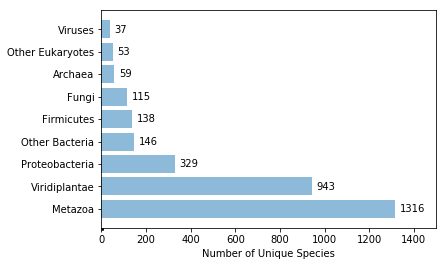
\includegraphics[width=100mm]{host_clades_figure.png}
            \caption{A breakdown of the kingdoms to which host species present in
            the database belong.}
            \label{host_clades_figure}
        \end{center}
    \end{figure}
    \begin{figure}[H]
        \begin{center}
            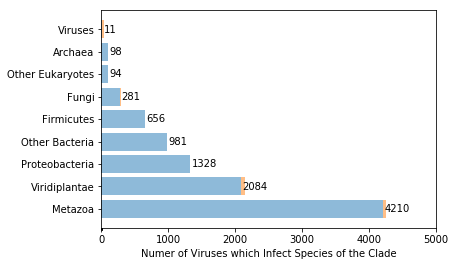
\includegraphics[width=100mm]{infects_clades_figure.png}
            \caption{A breakdown of viruses capable of infecting species of
            the given kingdom. The orange part represents viruses which can
            infect species of multiple kingdoms.}
            \label{infects_clades_figure}
        \end{center}
    \end{figure}

    Figure \ref{host_clades_figure} shows the vast majority of host species in
    the database are either animals (Metazoa) or plants (Viridiplantae). Fungal
    host species are relatively uncommon in the data.

    We see a similar pattern in the number of virus species that find their
    hosts in a given clade, as shown in Figure \ref{infects_clades_figure}.
    The numbers there are roughly proportional to those in Figure
    \ref{host_clades_figure}, save that plants seem to make up a somewhat
    proportionately smaller portion of the data. It also shows that viruses
    which are capable of infecting species belonging to more than one distinct
    kingdom are extremely rare in the data set; thus, we can effectively ignore
    this overlap.

    These figures show a very small number of fungal species and fungal viruses
    present in the database. While there are a number of domesticated species of
    fungus, and a comparison involving these and their wild counterparts may
    prove useful to this investigation, this relatively small degree of data
    on the subject resulted in the decision to exclude fungal species and their
    viruses from the rest of the investigation, and focus solely on plants and
    animals.
    



\end{document}